%%%%%%%%%%%%%%%%%%%%%%%%%%%%%%%%%%%%%%%%%%%%%%%%%%%%%%%%%%%%%%%%%%%
\documentclass[10pt,landscape]{article}
\usepackage{amssymb,amsmath,amsthm,amsfonts}
\usepackage{multicol,multirow}
\DeclareMathOperator*{\argmax}{arg\,max}
\DeclareMathOperator*{\argmin}{arg\,min}
\usepackage{calc}
\usepackage{tikz}
\usepackage{ifthen}
\usepackage{textcomp}
\usepackage{xcolor}
\usepackage{graphicx}
\usepackage{makecell}
\graphicspath{ {./images/} }
\usepackage{enumitem}
\usepackage{bm}
\usepackage{titlesec}
\usepackage[landscape]{geometry}
\usepackage{fancyhdr}
\usepackage[colorlinks=true,citecolor=blue,linkcolor=blue]{hyperref}
%------------------------------------
\ifthenelse{\lengthtest { \paperwidth = 11in}}
    { \geometry{top=.4in,left=.5in,right=.5in,bottom=.4in} }
	{\ifthenelse{ \lengthtest{ \paperwidth = 297mm}}
		{\geometry{top=1cm,left=1cm,right=1cm,bottom=1cm} }
		{\geometry{top=1cm,left=1cm,right=1cm,bottom=1cm} }
	}
\pagestyle{fancy}
\fancyhf{}
% Remove line
\renewcommand{\headrulewidth}{0pt}
\cfoot{\fontsize{9pt}{11pt}\selectfont Frank Facundo}
\setlength{\footskip}{16pt} % amount to move footer by
% Remember to call your parents and tell them you love them!

% Define smaller plus sign
\newcommand{\plus}{\raisebox{.3\height}{\scalebox{.7}{+}}}

\makeatletter
\renewcommand{\section}{\@startsection{section}{1}{0mm}%
                                {-1ex plus -.5ex minus -.2ex}%
                                {0.5ex plus .2ex}%x
                                {\normalfont\large\bfseries}}
\renewcommand{\subsection}{\@startsection{subsection}{2}{0mm}%
                                {-1ex plus -.5ex minus -.2ex}%
                                {0.5ex plus .2ex}%
                                {\normalfont\normalsize\bfseries}}
\renewcommand{\subsubsection}{\@startsection{subsubsection}{3}{0mm}%
                                {-1ex plus -.5ex minus -.2ex}%
                                {1ex plus .2ex}%
                                {\normalfont\small\bfseries}}
\makeatother
\setcounter{secnumdepth}{0}
\setlength{\parindent}{0pt}
\setlength{\parskip}{0pt plus 0.5ex}
% ----------------------------------------------------

\title{Linear Algebra}
\begin{document}

\raggedright
\footnotesize

\begin{center}
    \vspace{-50mm}
    \Large{\vspace{-15mm}\textbf{Linear Algebra}} \\
    \footnotesize{Last Updated \today}
    \vspace{-.4mm}
\end{center}
\begin{multicols}{3}
    \setlength{\premulticols}{1pt}
    \setlength{\postmulticols}{1pt}
    \setlength{\multicolsep}{1pt}
    \setlength{\columnsep}{2pt}
    % --------------------------------------------------------------
    \section{Concepts}
    \textbf{Determinant} - $det(A)$

    \textbf{Singular matrix} - $det(A)=0$
    
    \section{Vector Spaces and Subspaces}
    \subsection{Four Subspaces}
    Let $A$ a $m$ by $n$ matrix
    \smallskip
    \begin{center}
        \vspace{-1mm}
        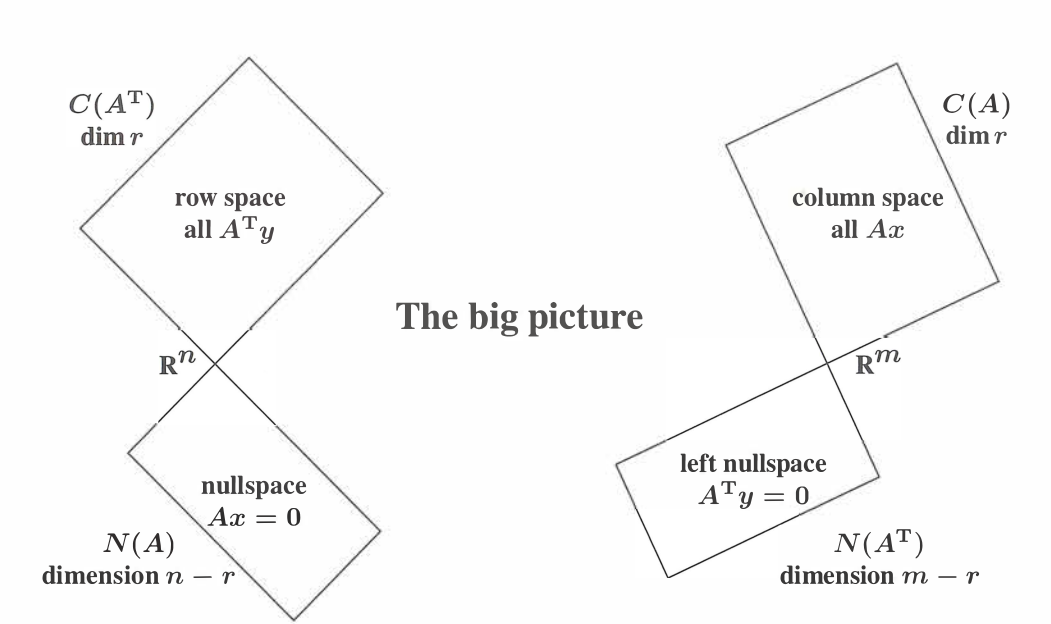
\includegraphics[scale = .2]{images/four_foundamental_subspaces.png}
    \end{center}
    \vspace{-2mm}
    \begin{itemize}
        \item $r=rank(A)=dim(C(A))= \text{Number of pivots}$
        \item $N(A)=$ Null space of $A=Ker(A)=$(FR) Noyau de $A$
        \item $C(A)=$Column Space of $A=Im(A)=$(FR) Image de $A$
    \end{itemize}
    \subsection{Fundamental Theorem of Linear Algebra}
    \begin{itemize}
        \item The column space and row space both have dimension $r$.
        \item The nullspaces have dimension $n-r$ and $m-r$
        \item $N(A)$ is the orthogonal complement of the row space $C(A^T)$ (in) $\mathbb{R}^n$
        \item $N(A^T)$ is the orthogonal complement of the column space $C(A)$ (in) $\mathbb{R}^m$
    \end{itemize}
    
    \columnbreak

    \section{Least Squares}
    \smallskip
    \begin{center}
        \vspace{-1mm}
        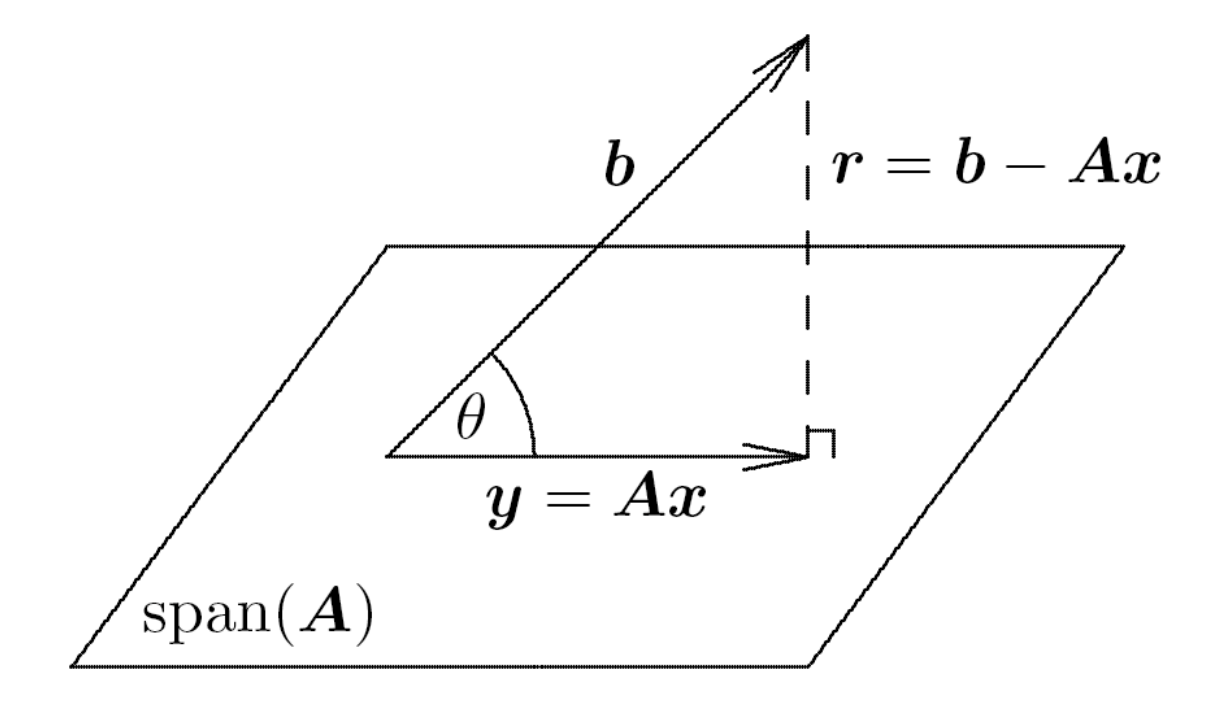
\includegraphics[scale = .15]{images/least_squares.png}
    \end{center}
    \vspace{-2mm}

    \begin{itemize}
        \item $span(A) \perp r$
        \item $span(A) = C(A) = Im(A)$
        \item $y \in span(A)$
    \end{itemize}
    $$\Rightarrow span(A) \perp r$$
    $$\text{because each column of A is perpendicular to r}$$
    $$\Leftrightarrow A^Tr = \vec{0}$$
    $$\Leftrightarrow A^T(b-Ax) = \vec{0}$$
    $$\Leftrightarrow x = (A^TA)^{-1}A^Tb$$
    $$\Leftrightarrow y = A(A^TA)^{-1}A^Tb$$
    $$\Leftrightarrow \rho = A(A^TA)^{-1}A^T$$
    $$\rho \text{ being the projection matrix}$$

    \columnbreak

    % \section{Eigenvalues and Eigenvectors}
    \section{Matrix factorizations}
    \begin{enumerate}
        \item $A=LU$
        \item $A=LDU$
        \item $PA=LU$
        \item $EA=R$
        \item $S=C^TC$
        \item $A=QR$ - orthonormal columns in Q, upper triangular R
        
        \textbf{Requirements}
        
        \item $A=X\Lambda X^{-1}$ - Eigenvectors in X, eigenvalues in $\Lambda$
        \item $A=Q\Lambda Q^T$
        \item $A=BJB^{-1}$
        \item $A=U\Sigma V^{T}$ - SVD: (orthogonal $U$ is $m\times m$)($m\times n$ singular value matrix $\sigma_1, ..., \sigma_r$ on its diagonal)(orthogonal $V$ is $n \times n$)
        \item $A^+=V\Sigma ^+ U^{T}$ - Pseudoinverse
        \item $A=QS$
        \item $A=U \Sigma U^{-1}$
        \item $A=Q T Q^{-1}$

    \end{enumerate}

\end{multicols}

\end{document}
